\documentclass[12pt]{article}
\usepackage[a4paper,margin=1in]{geometry}
\usepackage[T1]{fontenc}
\usepackage[utf8]{inputenc}
\usepackage{graphicx}
\usepackage{booktabs}
\usepackage{enumitem}
\usepackage{setspace}
\usepackage{float}
\usepackage{xcolor}
\usepackage{amsmath}
\usepackage{array}

\title{\textbf{Mirror Reflection Agent: Structured Reliability Control for Scientific Reasoning with Pilot Mechanism Evidence}}
\author{Brook \\ Independent Researcher}
\date{}

\begin{document}
\maketitle
\onehalfspacing
\emergencystretch=2em

\begin{abstract}
Large language models are increasingly used in scientific workflows, yet their practical value remains constrained by unsupported certainty, weak handling of conditional evidence, and poor retention of prior corrections. We present Mirror Reflection Agent, a reliability-control architecture that separates candidate cognition from final output and inserts an explicit mirror-critique stage between them. The system constructs a structured intermediate state, critiques it with typed verdicts such as revise, retrieve, wait, diverge, and pass, and stores correction lineage and reusable strategy signals in memory. Unlike prompt-only self-refinement pipelines, the proposed architecture externalizes intermediate cognition and makes revision control auditable. We instantiate the design with scientific and commonsense knowledge layers, a deterministic critique module, project-local memory, optional dual-layer memory, and replayable run audits. We report pilot evidence from the current repository benchmark, where the dual-layer setting reduces premature convergence and improves correction retention relative to a local-only setting. The manuscript makes a bounded claim: the present implementation demonstrates a proof-of-mechanism for reliability control, while a larger science-facing benchmark with fuller ablations remains future work.
\end{abstract}

\noindent\textbf{Keywords:} reflective agents, reliability control, scientific reasoning, memory, uncertainty, metacognition

\section{Introduction}

Scientific use of large language models requires more than fluent answers. A useful system must distinguish strong evidence from weak prior knowledge, preserve source conditions, reduce unsupported certainty, and remember prior corrections without blindly repeating them. Existing agent pipelines often improve outputs by adding reflection, retrieval, or tool use, but they still leave three recurring problems: intermediate reasoning is not represented as an inspectable object, critique outcomes are not encoded as explicit control decisions, and prior corrections are not preserved as structured reusable lineage.

This paper addresses those gaps with Mirror Reflection Agent, a structured reliability-control architecture. Rather than directly producing a final answer, the system builds a candidate cognitive state, critiques it with a mirror layer, and then either revises, retrieves memory, diverges to a new scaffold, defers, or finalizes. The design is engineering-oriented and auditable. It does not claim subjective awareness, consciousness, or human-like introspection. Its core claim is narrower and testable: explicit cognitive state plus typed critique plus correction-lineage memory can improve reliability-oriented behavior in scientific and science-adjacent reasoning tasks.

The contribution of the present manuscript is intentionally bounded. We do not claim a broad AI-for-Science benchmark victory. We claim that the current implementation provides pilot mechanism evidence for a reliability-control architecture whose main value lies in state externalization, verdict-typed oversight, and memory-guided correction reuse.

\section{Results}

\subsection{Mirror Reflection Agent externalizes reliability control}

The architecture follows the control flow:

\begin{center}
\texttt{input $\rightarrow$ knowledge layers $\rightarrow$ cognition $\rightarrow$ mirror critique $\rightarrow$ revise/retrieve/diverge/wait/pass $\rightarrow$ output $\rightarrow$ memory write-back}
\end{center}

\begin{figure}[H]
\centering
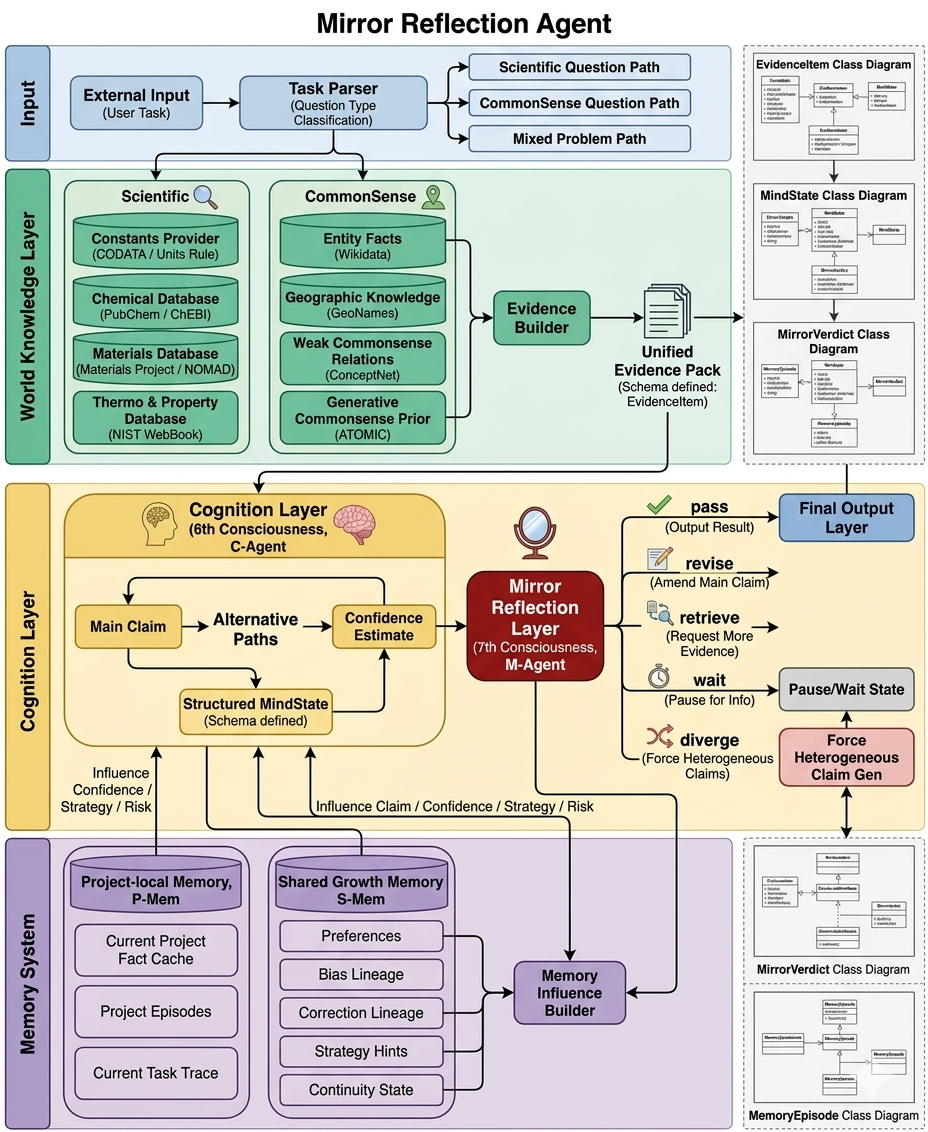
\includegraphics[width=\textwidth]{figure1_architecture.png}
\caption{Overall engineering schematic of Mirror Reflection Agent. The figure shows the relation between the scientific knowledge layer, commonsense knowledge layer, cognition layer, mirror reflection layer, and memory system.}
\label{fig:architecture-v3}
\end{figure}

The deepest contribution of the architecture is not generic self-reflection. It is the conversion of reliability problems into explicit state and explicit control flow. Candidate reasoning is represented as a structured \texttt{MindState}; critique is represented as a structured \texttt{MirrorVerdict}; and memory stores not only facts, but also prior bias alerts, correction actions, and reusable strategies. The contribution is therefore architectural rather than purely prompt-based.

This positioning matters because related reflective systems usually improve outputs through iterative refinement, retrieval, or verbal memory, but do not expose all of the same reliability-control components at once. Table~\ref{tab:positioning-v3} isolates the intended novelty of the present work.

\begin{table}[H]
\centering
\begin{tabular}{p{3.0cm}p{2.2cm}p{2.2cm}p{2.6cm}p{2.0cm}}
\toprule
Method & Externalized state & Typed control verdicts & Persistent correction lineage & Abstention governance \\
\midrule
Self-Refine & limited & no & no & no \\
Reflexion & partial & no & partial & limited \\
CRITIC & tool-grounded critique & no & no & limited \\
Self-RAG & retrieval-aware generation & partial & no & limited \\
Mirror Reflection Agent & explicit & yes & yes & yes \\
\bottomrule
\end{tabular}
\caption{Positioning of the present work against closely related reflective pipelines. The intended novelty is the combination of explicit state externalization, verdict typing, correction-lineage memory, and abstention-oriented control.}
\label{tab:positioning-v3}
\end{table}

\subsection{Pilot benchmark shows reliability-oriented gains}

We ran the existing repository benchmark without modifying the evaluation harness:

\begin{center}
\texttt{python3 -m evals.run\_evals --format json}
\end{center}

The pilot benchmark contains four cases and compares a \texttt{local\_only} configuration against a \texttt{dual\_layer} configuration. These cases target concept blending, premature convergence, project-local precedence, and bounded control behavior. All pilot metrics are computed by deterministic rules in the repository evaluation harness rather than by an external LLM judge. This makes the benchmark transparent and replayable, although narrower than a full-scale evaluation.

\begin{table}[H]
\centering
\begin{tabular}{lccc}
\toprule
Metric & local\_only & dual\_layer & delta \\
\midrule
Premature convergence rate & 1.000 & 0.000 & -1.000 \\
Revision success rate & 0.500 & 1.000 & +0.500 \\
Correction retention rate & 0.000 & 1.000 & +1.000 \\
Shared-memory pollution risk & 0.000 & 0.000 & 0.000 \\
Average confidence & 0.6075 & 0.5625 & -0.0450 \\
\bottomrule
\end{tabular}
\caption{Aggregate pilot benchmark results from the current implementation.}
\label{tab:pilot-aggregate-v3}
\end{table}

\begin{figure}[H]
\centering
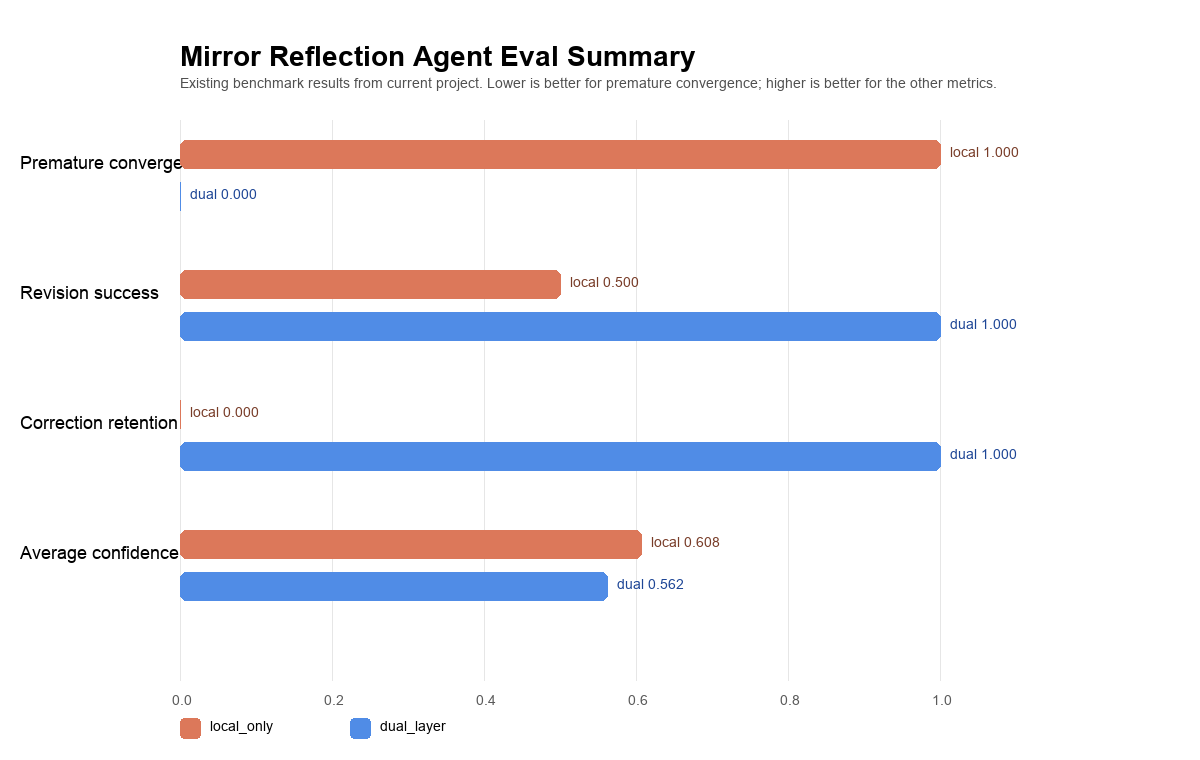
\includegraphics[width=\textwidth]{figure2_results.png}
\caption{Summary plot of the pilot benchmark. The dual-layer setting eliminates premature convergence in the current suite and substantially improves revision success and correction retention, while slightly reducing average confidence.}
\label{fig:pilot-summary-v3}
\end{figure}

Figure~\ref{fig:pilot-summary-v3} shows the core pilot result. The main gain is not that dual-layer memory makes the system more assertive. It makes the system more controlled. Premature convergence drops from 1.000 to 0.000, which means the architecture is less likely to lock into an overconfident conclusion too early. Revision success rises from 0.500 to 1.000, indicating that the mirror-plus-memory loop is not only triggering revisions but helping those revisions land in a safer final state. Correction retention rises from 0.000 to 1.000, supporting the central claim that structured correction lineage can influence later behavior in a measurable way. Average confidence decreases slightly from 0.6075 to 0.5625; in this setting that should be interpreted as improved calibration rather than degradation.

\subsection{Case-level analysis shows where the gains come from}

Aggregate metrics are useful but insufficient on their own. To make the mechanism visible, we also report case-level outcomes. The strongest effects appear in the two recovery-oriented cases: concept blending recovery and premature convergence alert. In those cases, dual-layer memory retains the relevant correction while the local-only setting does not.

\begin{table}[H]
\centering
\begin{tabular}{lcccc}
\toprule
Case & Mode & Verdict & Revisions & Correction retained \\
\midrule
Concept blending recovery & local\_only & pass & 1 & no \\
Concept blending recovery & dual\_layer & pass & 2 & yes \\
Premature convergence alert & local\_only & wait & 4 & no \\
Premature convergence alert & dual\_layer & wait & 4 & yes \\
Project-local precedence & local\_only & pass & 0 & yes \\
Project-local precedence & dual\_layer & pass & 0 & yes \\
Bounded control case & local\_only & pass & 0 & yes \\
Bounded control case & dual\_layer & pass & 0 & yes \\
\bottomrule
\end{tabular}
\caption{Case-level outcomes in the pilot benchmark.}
\label{tab:pilot-cases-v3}
\end{table}

\begin{figure}[H]
\centering
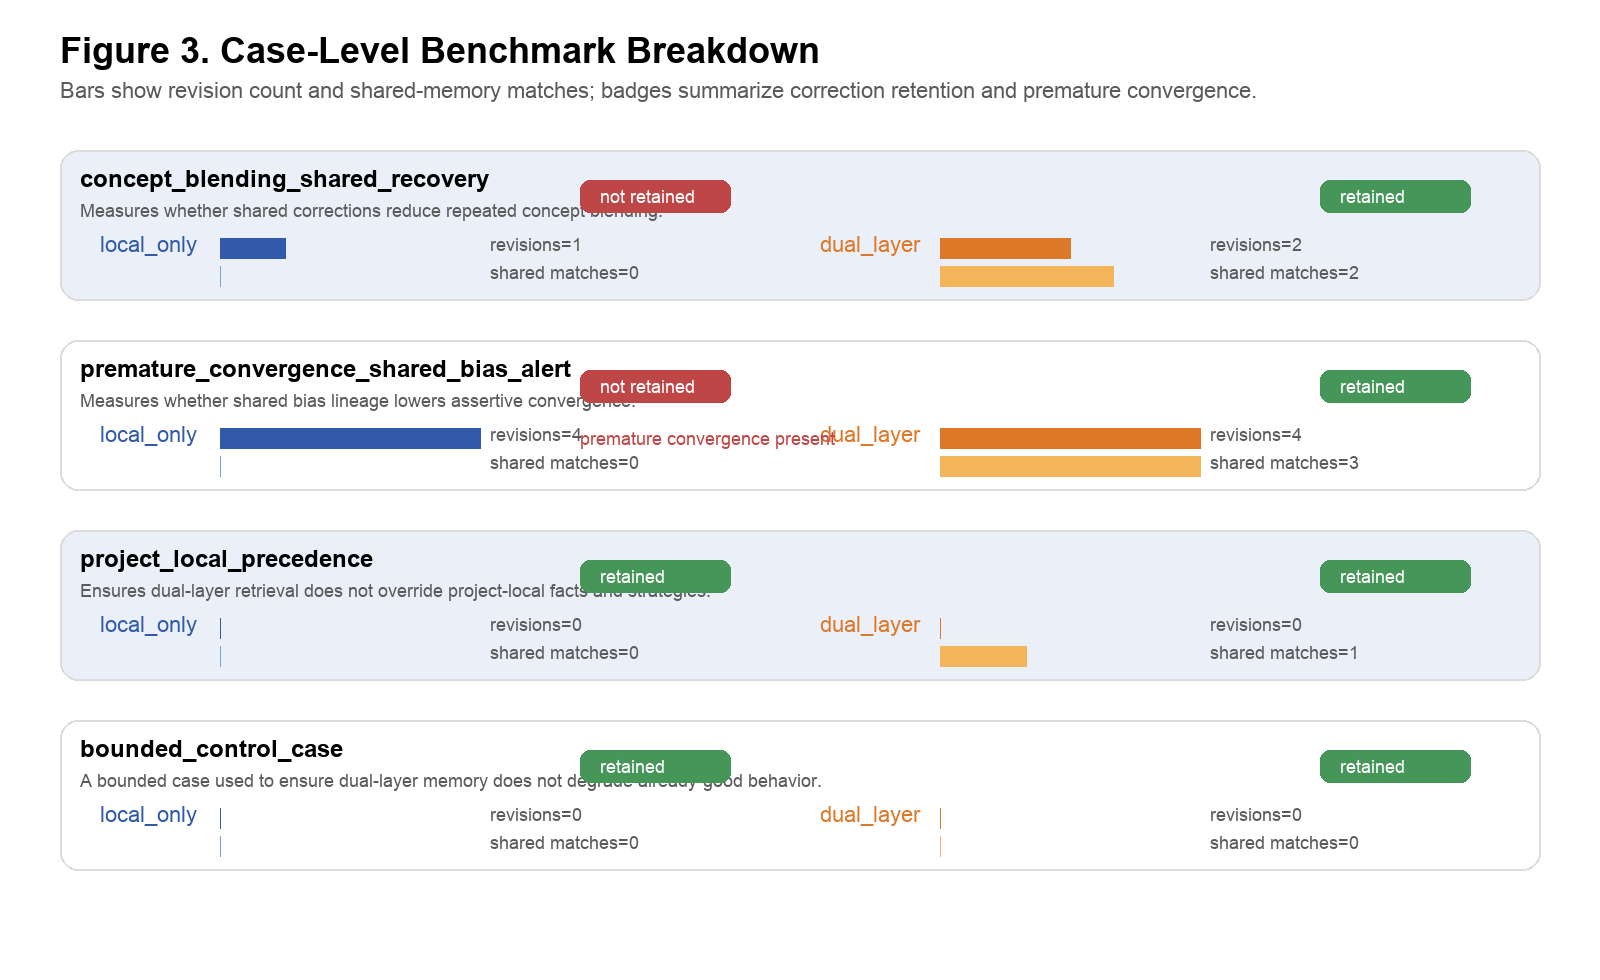
\includegraphics[width=\textwidth]{figure3_case_breakdown.png}
\caption{Case-level mechanism breakdown. Bars summarize revision counts and shared-memory matches, while badges indicate whether the target correction was retained.}
\label{fig:pilot-cases-v3}
\end{figure}

Figure~\ref{fig:pilot-cases-v3} and Table~\ref{tab:pilot-cases-v3} make the mechanism-level story more explicit. In the concept-blending case, dual-layer memory performs one additional revision and retrieves two shared matches, which is sufficient to retain the target correction while avoiding a stronger consciousness claim. In the premature-convergence case, both modes reach a \texttt{wait} verdict after four revisions, but only dual-layer memory retains the explicit shared correction and clears the premature-convergence flag. The remaining two cases show the boundary conditions of the architecture: project-local precedence is preserved, and already-bounded behavior is not degraded by the richer memory mode.

\subsection{Current pilot evidence is reproducible but still limited}

To check whether the pilot pattern is merely a one-off artifact, we repeated the benchmark for five iterations using the repository's built-in averaging mode:

\begin{center}
\texttt{python3 -m evals.run\_evals --iterations 5 --format json}
\end{center}

Across five iterations, the reported aggregate metrics remained unchanged. In the current implementation this indicates deterministic behavior under the pilot benchmark and supports the reproducibility of the present tables and figures. However, this repeated-run stability should not be over-interpreted. It demonstrates implementation-level reproducibility, not task-level statistical generalization.

\section{Discussion}

The present results support a narrow but useful claim: the architecture improves reliability-oriented behavior under correction and memory. They do not establish broad scientific superiority. The current benchmark is intentionally small, and the pilot should be read as evidence about control logic, not as evidence that the full scientific-knowledge envelope in Figure~\ref{fig:architecture-v3} has already been validated.

This is also where the paper's current limits become clear. The title and positioning invoke scientific reasoning, but the present benchmark is still closer to a reliability-mechanism suite than to a full science benchmark. The manuscript is strongest when it is read as a systems paper about inspectable reliability control with pilot evidence, rather than as a completed AI-for-Science evaluation paper.

At the same time, the pilot already demonstrates the type of gain that matters for this architecture. The system becomes less prone to premature commitment, more likely to preserve prior corrections, and more willing to trade raw confidence for bounded behavior. For a scientific assistant, that trade is desirable. A slightly less confident answer that respects evidence limits is often more valuable than a fluent but overgeneralized one.

The main implication is methodological. The architecture shows that some reliability gains can come from system design rather than foundation-model scale alone. That observation is particularly relevant in the context of local or modest-scale models, where explicit control may be more practical than relying exclusively on larger model families.

\section{Methods}

\subsection{System design}

Mirror Reflection Agent separates perception, cognition, critique, and memory into explicit layers. The cognition layer builds a structured \texttt{MindState} containing current input, task goal, main claim, evidence, hidden assumptions, alternative paths, confidence, self-risk, proposed action, and self-state. The mirror layer then emits a \texttt{MirrorVerdict} with one of five actions: \texttt{pass}, \texttt{revise}, \texttt{retrieve}, \texttt{wait}, or \texttt{diverge}. The memory layer stores facts, contexts, bias lineage, correction lineage, and reusable strategies. The current implementation is deterministic in control structure and logs cognition-to-mirror transitions for replayable audit.

\subsection{Implemented versus planned scope}

One source of potential confusion is the difference between the full architecture sketch and the subset exercised in the pilot benchmark. Table~\ref{tab:implemented-v3} separates the validated control loop from the larger system envelope.

\begin{table}[H]
\centering
\begin{tabular}{p{4.0cm}p{2.2cm}p{2.2cm}p{4.8cm}}
\toprule
Component & Status & Exercised in pilot & Current role \\
\midrule
Structured \texttt{MindState} generation & implemented & yes & candidate cognition state before final output \\
Typed mirror verdicts & implemented & yes & revise/retrieve/wait/diverge/pass control \\
Project-local memory & implemented & yes & correction and strategy retrieval \\
Shared-growth memory & implemented & yes & advisory cross-run correction support in dual-layer mode \\
Replayable audit trace & implemented & yes & reproducibility and case inspection \\
Scientific source routing ecosystem & partial / planned & not fully & intended evidence expansion for future science-facing benchmark \\
Large multi-source scientific QA workflow & planned & no & next-stage benchmark target rather than current validated scope \\
\bottomrule
\end{tabular}
\caption{Implemented versus planned scope of the architecture.}
\label{tab:implemented-v3}
\end{table}

\subsection{Pilot evaluation setup}

The pilot benchmark currently compares two settings: \texttt{local\_only} and \texttt{dual\_layer}. Each case seeds project-local and/or shared memory, runs the orchestrator, inspects the final \texttt{MindState} and \texttt{MirrorVerdict}, and computes deterministic metrics using the repository evaluation harness. The current benchmark includes four cases because its purpose is proof-of-mechanism rather than broad empirical coverage.

\subsection{Operational metric definitions}

Reviewer feedback correctly identified metric under-specification as a major weakness. Table~\ref{tab:metric-definitions-v3} therefore states the current operational definitions explicitly. These definitions are exact for the current implementation, even though they are not sufficient for a large-scale final benchmark.

\begin{table}[H]
\centering
\begin{tabular}{p{3.4cm}p{9.2cm}}
\toprule
Metric & Operational definition in the current harness \\
\midrule
Premature convergence rate & Fraction of designated premature-convergence cases whose final claim still triggers the mirror's premature-convergence detector. \\
Revision success rate & Fraction of cases requiring revision that both revise at least once and end in \texttt{pass} or \texttt{wait} with the target issue cleared. \\
Correction retention rate & Fraction of cases with an expected correction string whose final evidence or retrieved-lesson pool still contains that correction. \\
Shared-memory pollution risk & Fraction of shared-memory episode payloads in dual-layer mode that violate the harness' allowed value types or include project-specific contamination patterns. \\
Average confidence & Mean final \texttt{MindState.confidence} across cases. \\
\bottomrule
\end{tabular}
\caption{Operational definitions of pilot metrics.}
\label{tab:metric-definitions-v3}
\end{table}

\subsection{Reviewer-2-driven redesigned experiment protocol}

To address the strongest evaluation concerns, the next benchmark round should not simply add more cases. It should change the protocol in four specific ways.

\begin{enumerate}[leftmargin=1.4em]
\item \textbf{Complete the architecture-first ablation chain.} The comparison should include direct answer, structured cognition only, mirror without memory, mirror with local memory, and mirror with dual-layer memory.
\item \textbf{Expand task coverage.} The benchmark should include at least three task families: internal reliability cases, condition-sensitive scientific QA, and longitudinal correction cases.
\item \textbf{Specify metric and labeling rules.} Every metric should have a written rubric, a deterministic rule when possible, and stored raw outputs for audit.
\item \textbf{Release reproducibility assets.} The benchmark should publish prompts, seeded memory episodes, raw outputs, scoring scripts, and environment metadata.
\end{enumerate}

Table~\ref{tab:redesigned-benchmark-v3} summarizes the redesigned protocol intended to directly answer reviewer-2's criticisms about weak baselines, insufficient sample size, unclear metric definitions, and incomplete reproducibility.

\begin{table}[H]
\centering
\begin{tabular}{p{2.0cm}p{3.3cm}p{3.4cm}p{4.0cm}}
\toprule
Track & Task family & Required baselines & Core outputs \\
\midrule
Track A & internal reliability benchmark & direct answer, cognition only, mirror only, local memory, dual-layer memory & raw outputs, revision traces, issue flags, metric scores \\
Track B & condition-sensitive scientific QA & same architecture-first ablations & answer text, evidence pack, unit handling, abstention label, correctness label \\
Track C & longitudinal correction benchmark & local memory versus dual-layer memory plus direct answer reference & cross-session raw outputs, correction carryover, error recurrence, conflict cases \\
\bottomrule
\end{tabular}
\caption{Reviewer-2-driven redesigned benchmark protocol.}
\label{tab:redesigned-benchmark-v3}
\end{table}

\subsection{Reproducibility assets for the next version}

The current manuscript already includes replayable pilot assets in the local repository, including the single-run dump, repeated-run dump, case breakdown, and generated figures. A submission-ready next version should additionally provide the benchmark source file, the exact prompts used for all ablations, the seed memory payloads, the raw run outputs, a metric rubric document, and the environment and dependency snapshot used to reproduce the paper.

\section*{Data availability}

The implementation, pilot evaluation harness, manuscript sources, raw pilot outputs, and generated figures are maintained in the local project repository used for this study. The pilot metrics reported in this manuscript are reproduced from the repository evaluation commands described in the Methods section.

\section*{Code availability}

The current prototype and manuscript assets are stored in the local repository used to generate this draft. A submission-ready release should expose the exact benchmark cases, scoring logic, raw outputs, and environment snapshot needed to replay the pilot tables and figures.

\begin{thebibliography}{9}
\bibitem{selfrefine}
Madaan A, Tandon N, Clark P et al. 2023 Self-Refine: Iterative Refinement with Self-Feedback. arXiv:2303.17651.

\bibitem{reflexion}
Shinn N, Cassano F, Berman E and Labash B 2023 Reflexion: Language Agents with Verbal Reinforcement Learning. arXiv:2303.11366.

\bibitem{critic}
Gou Z, Shao Z, Gong Y et al. 2024 CRITIC: Large Language Models Can Self-Correct with Tool-Interactive Critiquing. arXiv:2305.11738.

\bibitem{selfrag}
Asai A, Wu Z, Wang Y et al. 2024 Self-RAG: Learning to Retrieve, Generate, and Critique through Self-Reflection. arXiv:2310.11511.

\bibitem{sofai}
Bergamaschi Ganapini M, Campbell M, Fabiano F et al. 2025 Fast, slow, and metacognitive thinking in AI. npj Artificial Intelligence 1, 27.

\bibitem{academicresponse}
Sun Z, Zhang Y, Liu X et al. 2025 Self-reflection enhances large language models towards substantial academic response. npj Artificial Intelligence 1, 45.
\end{thebibliography}

\end{document}
